\section{Definitions and Numerical Computations of Lyapunov Exponents}

One of the key defining properties of chaos in dynamical systems is that small perturbations in the initial conditions leads large difference overtime.
With the assumption that the distance of nearby points increases exponentially over time, the following simplistic formula for the dynamical system of an iterative map $F$ can be deduced
\begin{align}\label{eq:lyapunov_exponent}
    \left|F^n(x_0+\epsilon)-F^n(x_0)\right| \sim \epsilon e^{n \lambda}.
\end{align}
where $\lambda$ is the Lyapunov exponent \cite{nonlinear_system} \cite{lyapunov}, $x_0$ the point at discrete time $0$ and evolves by the relations $x_{n+1} = F(x_n)$.

A positive $\lambda$ means nearby points of $x_0$ will move away from it as time progresses, and a negative $\lambda$ means nearby points will converge to $x_0$. 
The absolute value of $\lambda$ denotes the rate of diverging or converging.

The existence of such $\lambda$ is not obvious, the analytical evaluation of $\lambda$ is often hopeless, and the assumption seems very questionable.
However, if acquiescing such a formula, $\lambda$ can be calculated numerically and give important insights of the dynamical system. 


Assuming that $\epsilon e^{nL} \to 0$ and $\epsilon$ is small, \eqref{eq:lyapunov_exponent} becomes
$$
\epsilon \left| \frac{dF^n(x_0)}{dx} \right| \sim \epsilon e^{nL}.
$$

By taking logarithm
\begin{align}
    \lambda 
    &= \lim_{n \to \infty}\left(\frac{1}{n}\ln{\left|\frac{dF^n(x_0)}{dx}\right|}\right)  \\
    &= \lim_{N \to \infty}\left\{\frac{1}{N}\sum_{n=0}^{N-1}\ln{|F'(x_n)|}\right\}  \label{eq:lambda}.
\end{align}
Where in the last step we have labelled the points $x_1 = F(x_0), x_2 = F(x_1), \dots$ and applied the chain rule.
All of the numerical calculations of Lyapunov exponents in this report will use formula \eqref{eq:lambda}.

The equation \eqref{eq:lambda} fails to make sense at the points $x$ where $F'(x) = 0$.
Such points are \emph{superstability} points, and the Lyapunov exponents of which are defined as $- \infty$.

The following are some examples of calculating Lyapunov exponents.

\begin{exmp}
	Let us the tent map defined in equation \eqref{eq:tent} and the dynamical system depending on one parameter $r$ generated by the iterations of it.
    \begin{align}
        F(r, x)= 
        \begin{cases}
            r x, & \text{ if } x \in [0,1/2) \\
            r (1-x), & \text{ if } x \in [1/2,1]
        \end{cases} \label{eq:tent}
    \end{align}
	By equation \eqref{eq:lambda}, the Lyapunov exponent at $0$ is $\ln r$, which is negative if $r < 1$ and positive otherwise.
	The higher subfigure of \ref{fig:lyapunov_tent} is the bifurcation diagram of the Tent map showing its dynamical properties. 
	It is obtained by selecting 1000 equally spaced $r \in [0,2]$, and for each $r$ picking a random starting point $x_0$, iterating $x_0$ for $1000$ times, ignoring the first $200$ iterations, and plotting the rest $800$ $ x_i$ as a faint blue dot at coordinate $(r, x_i)$. 
	There is a dramatic change in behavior exactly at $r=1$ where the Lyapunov exponent changed from negative to positive, before which all the $x_0$ converges to $0$, whereas afterwards the system shows an apparent chaotic behavior by casting an interesting homogeneous shape of doubly curved triangle.

    \begin{figure}
        \centering
        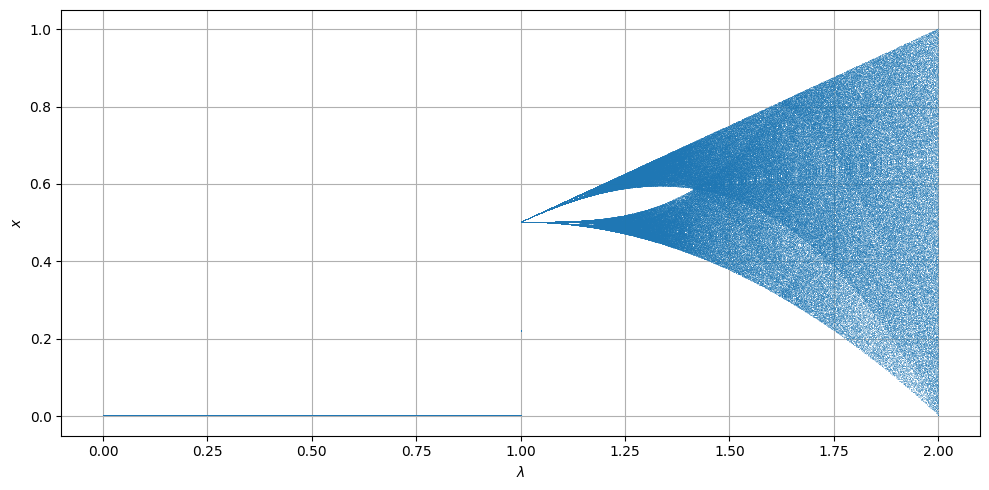
\includegraphics[width=\linewidth]{Bifurcation Images/Bifurcation_tent.png}
        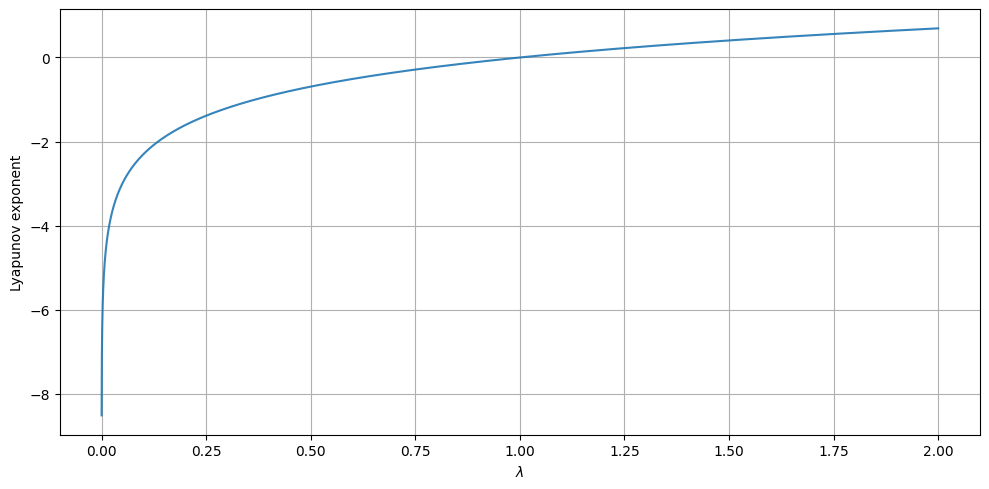
\includegraphics[width=\linewidth]{Bifurcation Images/Lyapunov_Tent.png}
        \caption{Bifurcation diagram and Lyapunov exponent plot for the tent map \eqref{eq:tent}}
        \label{fig:lyapunov_tent}
    \end{figure}
\end{exmp}

\begin{exmp}
	Similarly consider the dynamical system depending on one parameter $r$ generated by the iterations of the map
    $F(r,x)=x^2+r$ where $x,\lambda \in \mathbb{R}$.
	Unlike the case of tent map, there is no simple closed form for Lyapunov exponent, and computer simulations are required. 
	The bifurcation diagram and the Lyapunov exponent calculated with formula \eqref{eq:lambda} is shown in figure \ref{fig:lyapunov_x^2}.
    \begin{figure}
        \centering
        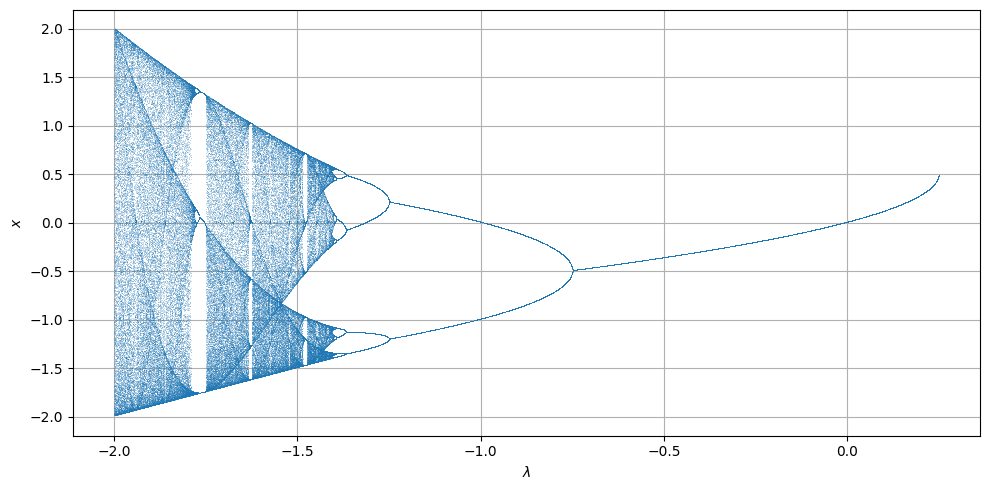
\includegraphics[width=1\linewidth]{Bifurcation Images/bifurcation_x^2.png}
        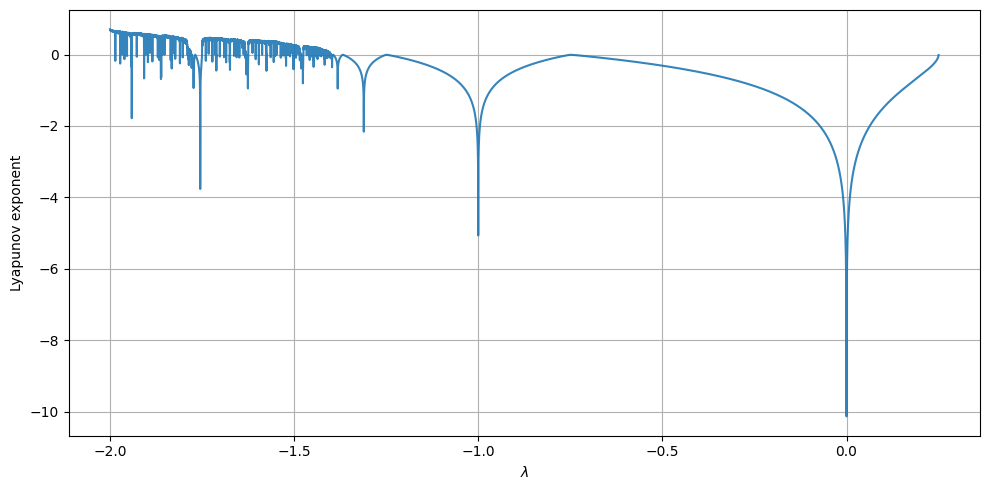
\includegraphics[width=1\linewidth]{Bifurcation Images/lyapunov_x^2.png}
        \caption{Bifurcation diagram and Lyapunov exponent plot for the map $F(\lambda,x)=x^2+\lambda$}
        \label{fig:lyapunov_x^2}
    \end{figure}
	A very interesting phenomenon of periodic doubling is apparent from the bifurcation diagram (which is studied in detail in chapter \ref{chapter:bifurcation}).
	Similar to the tent map, regions when the Lyapunov exponent is negative corresponds to distict lines in the bifurcatio diagram, while those with positive Lyapunov exponent corresponds to chaotic bands.
\end{exmp}




\section{Lyapunov Exponents for a Continuous Time Series}

Previously we have discussed the implications and how we solved for the Lyapunov exponent in discrete dynamical systems. 
But, if we consider continuous time dynamical systems in multiple dimensions, we observe something different. 
For continuous systems we need to consider the complete spectrum of lyapunov exponents which utilizes spectral calculations. 
Given a continuous dynamical system in an $n$-dimensional phase space, we monitor the long-term evolution of an infinitesimal $n$-sphere of initial conditions. 
It quantifies the average exponential growth or decay rates of perturbations in different directions in phase space. 
For an $n$-dimensional system, the Lyapunov spectrum consists of $n$ exponents, $L_1 \geq L_2 \geq \dots \geq L_n$, which describe the system's behavior in terms of expanding, neutral, and contracting directions.

Lets consider a continuous-time dynamical system defined by
$$
\dot{\mathbf{x}}(t) = \mathbf{f}(\mathbf{x}(t)),
$$
where $\mathbf{x}(t) \in \mathbb{R}^n$ is the state vector, and $\mathbf{f}$ is a smooth vector field. To study the evolution of perturbations, we linearize the system around a reference trajectory $\mathbf{x}(t)$. The evolution of a small perturbation $\delta\mathbf{x}(t)$ is governed by the linearized dynamics:
$$
\dot{\delta\mathbf{x}}(t) = \mathbf{J}(\mathbf{x}(t)) \delta\mathbf{x}(t),
$$
where $\mathbf{J}(\mathbf{x}(t))$ is the Jacobian matrix of $\mathbf{f}$ evaluated at $\mathbf{x}(t)$:
$$
\mathbf{J}(\mathbf{x}(t)) = \frac{\partial \mathbf{f}}{\partial \mathbf{x}} \bigg|_{\mathbf{x}(t)}.
$$
The $i$-th Lyapunov exponent $L_i$ is thus defined as:
\begin{align}
    L_i = \lim_{t \to \infty} \frac{1}{t} \log_2 \frac{p_i(t)}{p_i(0)}, \label{eq:continuous}
\end{align}
where $p_i(t)$ is the length of the $i$-th principal axis of an infinitesimal $n$-sphere of initial conditions evolved under the flow. The Lyapunov exponents describe the long-term exponential growth rates of perturbations in different directions.

An infinitesimal $n$-sphere of initial conditions evolves into an $n$-ellipsoid due to the locally deforming nature of the flow. The principal axes of the ellipsoid grow or shrink at rates determined by the Lyapunov exponents. A positive exponent ($L_i > 0$) indicates expansion in the corresponding direction. A zero exponent ($L_i = 0$) indicates a neutral direction, such as along the flow of a trajectory. A negative exponent ($L_i < 0$) indicates contraction in the corresponding direction.

From \eqref{eq:continuous} we can see that the ellipsoid grows with a rate of $2^{L_1t}$. The area is defined by the first 2 principle axis $2^{(L_1+L_2)t}$, and the volume by the third, $2^{(L_1+L_2+L_3)t}$. Thus in $n$-dimensional space volume of the ellipsoid evolves as
$$
V(t) \sim 2^{(L_1 + L_2 + \dots + L_n)t}.
$$
For dissipative systems, a system that releases energy instead of retaining it, the sum of the Lyapunov exponents is negative, indicating that the volume of the ellipsoid contracts over time.

In 3 dimensions, the sum of all the Lyapunov exponents is equivalent to the trace of the systems corresponding Jacobian matrix. 
The possible Lyapunov spectra and the corresponding attractors are $(+,0,-)$ which signifies a strange attractor or chaotic behavior. 
In order for the system to be chaotic only one of the individual exponents needs to be positive. 
$(0,0,-)$ tells us that the system will demonstrate quasi-periodic behavior. 
$(0,-,-)$ corresponds to the presence of a limit cycle or periodic behavior. 
Finally $(-,-,-)$ telling us that there is a stable fixed point. 
The sum of the Lyapunov exponents equals the time-averaged divergence of the phase space velocity. 
The value indicates the divergence of the flow and is the fractional rate of the volume expansion or contraction of the system, but for a conservative or Hamiltonian system this sum is zero. 
For dissipative systems, this sum is negative, ensuring that at least one exponent is negative. 
As a result, the long-term motion of trajectories converges to a limit set with zero volume, known as an attractor. 
While Lyapunov exponents are defined based on long-time averages, short trajectories may not fully capture the distinct behaviors associated with positive, zero, and negative exponents.

% To compute the Lyapunov spectrum numerically, we start by linearising the system by solving for the Jacobian matrix $\mathbf{J}(\mathbf{x}(t))$ along the reference trajectory $\mathbf{x}(t)$. We then need to evolve the perturbation vectors. We need to initialize a set of $n$ orthonormal perturbation vectors $\{\mathbf{v}_1, \mathbf{v}_2, \dots, \mathbf{v}_n\}$ and evolve them using the linearised dynamics
% $$
% \dot{\mathbf{v}}_i(t) = \mathbf{J}(\mathbf{x}(t)) \mathbf{v}_i(t).
% $$
% Subsequently we need to use the Gram Schmidt reorthonormnalisation on the vector frame that we created in order to to maintain their independence and prevent numerical overflow. Then we can track the growth rates of the perturbation vectors and accumulate their logarithmic growth rates
% $$
% \sum_{i=1}^n \ln \|\mathbf{v}_i(t)\|.
% $$
% where the Lyapunov exponents are computed as the time-averaged logarithmic growth rates
% $$
% L_i = \lim_{t \to \infty} \frac{1}{t} \ln\frac{\|\mathbf{v}_i(t)\|}{\|\mathbf{v}_i(0)\|}.
% $$


The Lyapunov spectrum is closely related to the fractal dimension of the attractor. The Kaplan–Yorke conjecture uses Lyapunov exponents to deduce the dimension of an attractor within a dynamical system. In order to quantify the complexity of chaotic attractors, which often exhibit fractal structure, Lyapunov exponents are able help provide information about the system's dynamics, while fractal dimension characterises the geometry of the attractor. The conjecture is able to link these two concepts together. The conjecture is based on the idea that the sum of Lyapunov exponents relates to the expansion and contraction rates of phase space volumes. The fractal dimension is then estimated by balancing the cumulative expansion (positive Lyapunov exponents) against the cumulative contraction (negative Lyapunov exponents). Let us arrange the Lyapunov exponents from largest to smallest such that $L_1 \geq L_2 \geq \dots \geq L_n$. Let $k$ thus be the largest index in which
$$
\sum_{i=1}^k L_i\geq 0 \quad\quad \text{ and } \quad \quad \sum_{i=1}^{k+1} L_i <0
$$
The Kaplan-Yorke dimension, defined as
$$
D = k + \frac{\sum_{i=1}^k L_i}{|L_{k+1}|},
$$
where $k$ is the largest integer such that $\sum_{i=1}^k L_i \geq 0$ which provides an estimate of the fractal dimension.

\begin{exmp}
    \begin{figure}
        \centering
        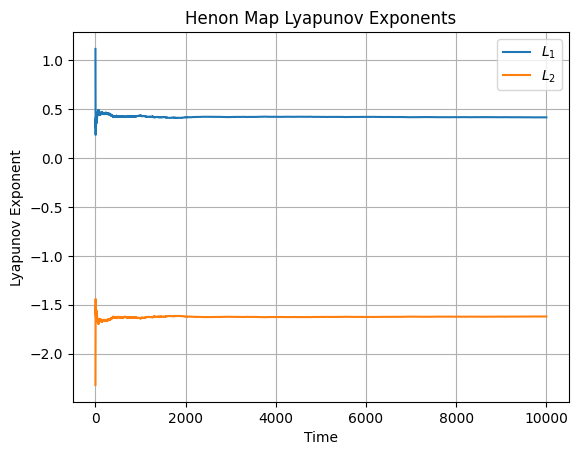
\includegraphics[width=0.95\linewidth]{Bifurcation Images/lyapunov_henon.png}
        \caption{Caption}
        \label{fig:lyapunov_henon}
    \end{figure}
    Lyapunov exponents base e: 0.41762663136121125 -1.6215994356871315
    Lyapunov exponents base 2: 0.6025078700079933 -2.339473464174202
\end{exmp}

% Given a continuous dynamical system in an $n$-dimensional phase space, we monitor the long-term evolution of an infinitesimal $n$-sphere of initial conditions. The sphere will become an $n$-ellipsoid due to the locally deforming nature of the flow. The $i$th one-dimensional Lyapunov exponent is then defined in terms of the length of the ellipsoidal principal axis $p_i(t)$
% \begin{align}
%     L_i=\lim_{n \to \infty} \frac{1}{n}\log_2\frac{p_i(t)}{p_i(0)} \label{eq:continous}
% \end{align}
% where $L_i$ are the individual exponents. Thus the Lyapunov exponents are related to the expanding or contracting nature of different directions in phase space. Since the orientation of the ellipsoid changes continuously as it evolves, the directions associated with a given exponent vary in a complicated way through the attractor. One cannot, therefore, speak of a well-defined direction associated with a given exponent. From \eqref{eq:continous} we can see that the ellipsoid grows with a rate of $2^{L_1t}$. The area is defined by the first 2 principle axis $2^{(L_1+L_2)t}$, and the volume by the third$2^{(L_1+L_2+L_3)t}$. From this we can create a new definition for the spectrum of exponents, the sum of the first $j$ exponents is define by the long term exponential growth rate of a $j$-volume element. This will provide us with a basis for the spectra technique fro experimental data.

% Any continuous time dependent dynamicla system without a fixed point will have at least one zero exponent which links with the slowly changing magnitude of a principle axis  tangent to the flow

% In a three-dimensional continuous dissipative dynamical system the only possible spectra, and the attractors they describe, are as follows: $( + , 0 , - )$ , a strange attractor; $(0,0,-)$, a two-toms; $(0, - , -)$, a limit cycle; and $( - , - , - )$ , The sum of each individual exponents is the time-averaged divergence of the phase space velocity; hence any dissipative dynamical system will have at least one negative exponent, the sum of all of the exponents is negative, and the post transient motion of trajectories will occur on a zero volume limit set, an attractor. Since Lyapunov exponents involve long-time averaged behavior, the short segments of the trajectories shown in the figure cannot be expected to accurately characterize the positive, zero, and negative exponents; nevertheless, the three distinct types of behavior are clear.

% The Lyapunov spectrum is closely related to the fractional dimension of the associated strange attractor.
%--------------------------------------------------------------------------------------------------%

% \textbf{Show that the $p$-cycle $\{X_1, X_2, \dots, X_p\}$ of the continuously differentiable map $F: \mathbb{R} \to \mathbb{R}$ is stable if  
% \[
% | F'(X_1) F'(X_2) \dots F'(X_p)| < 1.
% \]
% This is a proof the textbook refers to a lot in the section and I dont know how to interpret it or include it.}


% Idea: If we have an initial condition $x_0$ which will generate our sequence for a distcete dynamical system to use discrete time, and a point nearby $x_0 + \epsilon_0$. Let $\epsilon_n$= separation of orbits from $x_0$ and orbit from $x_0 + \epsilon_0$

% If $|\epsilon_n| \sim |\epsilon_0|e^{n\lambda}$ is converging exponentially, $\lambda$ is they lyanopunov exponent
% -$\lambda>0$ means chaos